\input{/home/diego/Documents/Licenciatura/LatexBasic/Preamble_general}

%%%%%%%%%%%%%%%%%%%%%%%%%%%%%%%%%%%%%%%%%%%%%%%%%%%%%%%%%%%
\usepackage{fancyhdr}%formato de pagina
\pagestyle{fancy}%colocar la pagina con el formato deseado
\fancyhead{}
\fancyhead[L]{\footnotesize{Electrónica Digital}}
\fancyhead[C]{Tarea 2}
\fancyhead[R]{\footnotesize{\thepage}}
%\fancyhead[LO,RE]{Cálculo 3}
%\fancyhead[RO,LE]{\footnotesize{\thepage}}
\fancyfoot{}
\fancyfoot[L]{Diego Sarceño}
%\fancyfoot[LO,RE]{Diego Sarceño}
%%%%%%%%%%%%%%%%%%%%%%%%%%%%%%%%%%%%%%%%%%%%%%%%%%%%%%%%%%%

\begin{document}
\begin{titlepage}
% AUTOR: Diego Sarceño

% ENCABEZADO DE TRABAJOS CON LOGO DE LA UNIDAD ACADÉMICA

% ENCABEZADO LOGO COLOR
%\begin{tabulary}{20cm}{Lp{0.9cm}p{6.1cm}}
%Universidad de San Carlos de Guatemala & & \multirow{4}{8cm}{\hfill %\includegraphics[scale=0.5]{ECFM.png}}\\            % Logo de la unidad academica
%Escuela de Ciencias Físicas y Matemáticas & \hfill & \\
%Diego Sarceño 201900109 & \hfill & \\
%Análisis de Variable Compleja 1 & \hfill & \\
%\today & & \\
%\end{tabulary}\\[0.25cm]


% ENCABEZADO LOGOS
\begin{tabulary}{20cm}{LLCRR}
\multirow{4}{2.3cm}{\includegraphics[scale=0.13]{/home/diego/Documents/Licenciatura/LatexBasic/ECFM.pdf}} & Universidad de San Carlos de Guatemala  & & & \multirow{4}{5cm}{\hfill \includegraphics[scale=0.082]{/home/diego/Documents/Licenciatura/LatexBasic/USAC.pdf}}\tabularnewline
 & Escuela de Ciencias Físicas y Matemáticas & \hfill &  & \tabularnewline
 & Mecánica 3 & \hfill ~~ &   & \tabularnewline
 & Diego Sarceño 201900109 & &  & \tabularnewline
 & \today &  & & \tabularnewline
\end{tabulary}\\[0.75cm]

{\hrule height 1.5pt} \vspace{0.1cm}
\begin{tabulary}{21cm}{p{6cm}p{7cm}p{8cm}}
    \hfill & \huge{\scshape{Tarea 4}} & \hfill
\end{tabulary}
{\hrule height 1.5pt} 
\vspace{0.5cm}


\noindent
El circuito se puede simular con este link (estará habilitado por $14$ días):	\href{https://www.tinkercad.com/things/cv6sa2X4fHt-epic-lappi-snicket/editel?sharecode=3q_45UNZrDWtQPS0XWcOTyARk8tDUIB1IFiOFfVmGVs}{TinkerCad}.
\\
El archivo de \LaTeX esta disponible en el repositorio de \href{https://github.com/DSarceno/Semestre6/tree/main/Electr\%C3\%B3nica\%20Digital/Tarea\%202}{GitHub}.


 % Tarea 1 ED
 

\section{Bitácoras}

\subsection{Bitácora 1}
Se inicio con una compuerta XOR en \textit{TinkerCad} la cual me dio problemas por el hecho de que no concuerda con la tabla de verdad, cada una de las entradas se hicieron con un pull up y un pull down respectivamente.

\subsection{Bitácora 2}
Se arreglo el error en la entrada del pull up, el LED está encendido sin necesidad de presionar el push button. La tabla de verdad para XOR y la tabla de verdad obtendida con el circuito es:

\begin{table}[H]
	\centering
	\caption{Tabla de datos obtenida por el circuito \ref{XORi}. (XOR)}
	\label{XOR}
	\begin{tabular}{||c|c||c|c||}
		\hline
		\hline
		\multicolumn{2}{||c||}{INPUT} & EXPECTED OUTPUT & RESULT OUTPUT \\
		\hline
		\hline
		$0$ & $0$ & $0$ & $0$ \\
		$0$ & $1$ & $1$ & $0$ \\
		$1$ & $0$ & $1$ & $1$ \\		
		$1$ & $1$ & $0$ & $0$ \\
		\hline
		\hline
	\end{tabular}
\end{table}

\begin{figure}[H]
	\centering
	\label{XORi}
	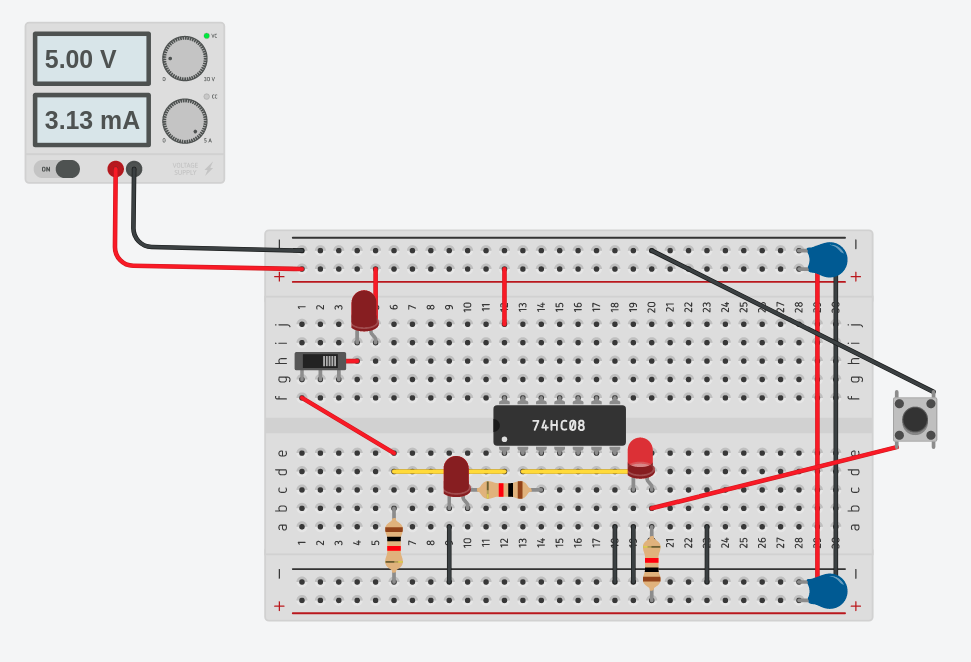
\includegraphics[scale=0.25]{Images/XOR.png}
	\caption{Circuito que modela la operación binaria XOR.}
\end{figure}


\subsection{Bitácora 3}

Se realizo la compuerta AND, también con una entrada pull up y una pull down. Con esto, en la pull up, se tenía problemas con el LED, así que se obvio dicho LED y se hicieron las respectivas pruebas. Lo cual resultó en la compuerta deseada:

\begin{figure}[H]
	\centering
	\label{ANDi}
	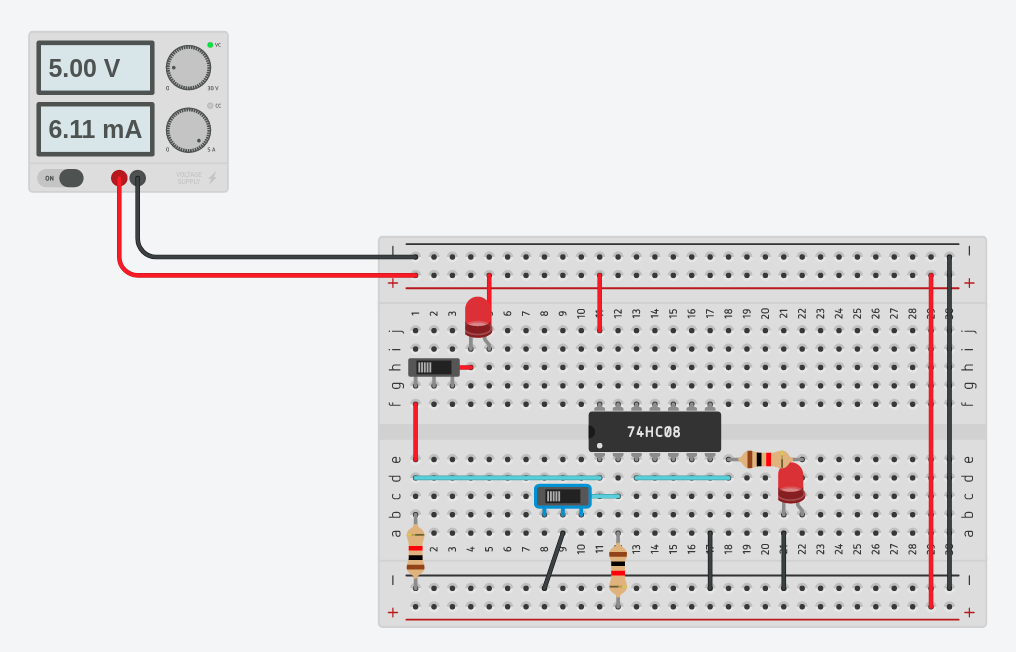
\includegraphics[scale=0.4]{Images/AND.png}
	\caption{Circuito de compuerta AND con entradas pull up y pull down.}
\end{figure}


\begin{table}[H]
	\centering
	\caption{Tabla de datos obtenida por el circuito \ref{ANDi}. (AND)}
	\label{XOR}
	\begin{tabular}{||c|c||c|c||}
		\hline
		\hline
		\multicolumn{2}{||c||}{INPUT} & EXPECTED OUTPUT & RESULT OUTPUT \\
		\hline
		\hline
		$0$ & $0$ & $0$ & $0$ \\
		$0$ & $1$ & $0$ & $0$ \\
		$1$ & $0$ & $0$ & $0$ \\		
		$1$ & $1$ & $1$ & $1$ \\
		\hline
		\hline
	\end{tabular}
\end{table}














































\end{titlepage}
\end{document}
